\section{Laboratory work implementation}

\subsection{Tasks and Points}

\begin{itemize}
	\item Aplicatia trebuie sa fie dezvoltata si testata cu orice SDK ce include Emulator
	\item Testarea aplicatiei pe un device real
	\item Aplicatia trebuie sa suporte device-urile cu diferite rezolutii
	\item Realizeaza o aplicatie care va implimenta tehnica Pomodoro
	\item Foloseste libraria cross platform pentru a realiza o apliacatie cross platform (aplicatia poate fi compilata atit pe Android, cit si pe iOS)
\end{itemize}

\subsection{Analiza lucrarii de laborator}

Repository \url{https://github.com/dragosh1011/MIDPS-laboratories/tree/master/MIDPS/LAB_4}{link}

Primul pas în elaborarea aplicației a fost alegerea unui sdk. Am optat pentru ionic 2\cite{ionic}, deoarece permite compilare pentru diferite dispozitive și este bazat pe ultimele tehnolgii, utilizînd angular 2 și typescript. Următorul pas a fost generarea unui template automat și analizarea lui, precum și trecerea rapidă prin documentație pentru a ști ce componente pot utiliza la dezvoltarea aplicațieie și prin ionic-cli\cite{ionic-cli} pentru a vedea cum se face emularea aplicației și care este modul de dezvoltare.

Al doilea pas a fost documentarea despre tehnica promodoro\cite{promodoro} și determinarea componentelor necesare. 

După aceste etape am putut să încep procesul de dezvoltare a aplicației. Mai întîi am creat prima pagina care reprezintă o listă de butoane care permit trecerea pe paginile cu fiecare tip de taskuri in parte precum și butonul care deschide pagina de creare a unui task. Prima problemă pe care am întîlnit-o a fost lipsa cunoștințelor suficiente în angular 2\cite{angular2} și diferențele majore față de angular 1. De asemenea, am avut careva dificultăți cu limbajul typescript care nu are un tip de date Object. Crearea unui service pentru taskuri a fost urmaorul pas, astfel încît taskurile să fie stocate întrun singur loc și să fie în aceiași stare în toate componentele aplicației. 

Divizarea taskurilor se face în:
\begin{itemize}
	\item Today - taskurile care sunt marcate pentru efectuare astăzi
	\item History - lista taskurilor finisate
	\item Inventory - lista taskurilor planificate
\end{itemize}

Un task are structura: 
\begin{itemize}
	\item id - un simplu unic identifier care reprizinta valoarea functie Date.now()
	\item status - lunul din tipurile enumerate mai sus
	\item promodoros - numărul de promodoros care au fost utilizate pentru finisarea taskului
	\item createdAt - data crearii
	\item ebdedAt - data finisarii
\end{itemize}

Urmatorul pas a fost crearea unei pagini simple pentru adaugarea de noi taskuri. Pagina respectiva este formata din titlu, inpu pentru titlu si putoane pentru intorcerea pe pagina inițială și buton pentru crearea taskului. 

Crearea paginii promodoro si a timerului a fost cea mai complicata parte a procesului de dezvoltare. Timerul a fost creat ca o componenta separata care este inclusă în pagina promodoro. Aceasta componenta primeste ca parametru numarul de secunde in care se finiseaza actiunea si ofera ca output evenimente ce pot fi ascultate pentru inceputul si sfirsitul secundamerului. 
Aici deosebim 4 stari in care se poate afla pagina:
\begin{itemize}
	\item lucrul la task - timp 25 min
	\item pauza normala - 5 min
	\item pauza lunga - 15 min dupa fiecare al 4-lea task indeplinit
	\item nedumerire - intrebare utilizatorului dupa ce un ciclu de promodoro + break a fost finisat, daca continua lucrul la acest task sau taskul este finisat.
\end{itemize}

Ultima etapă a fost de a testa aplicația creată pe un emulator, apoi si pe un dispozitiv mobil.

\break
\subsection{Imagini}

\begin{center}
	\begin{figure}[h]
		\centering
		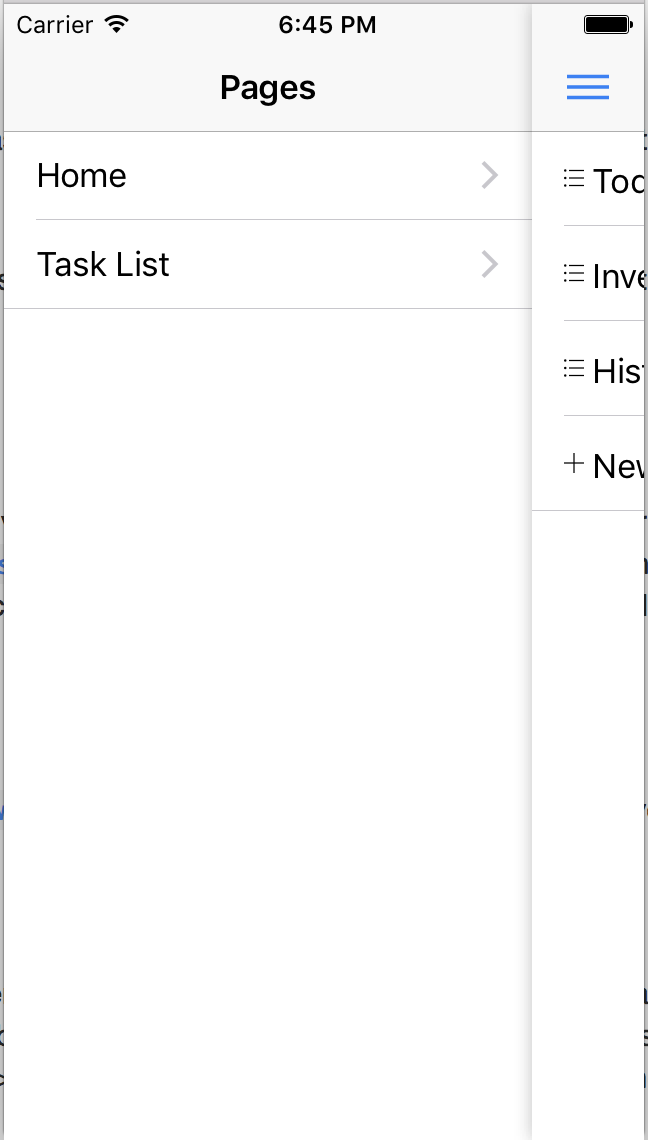
\includegraphics[width=10cm]{menu}\\
		\caption{Menu}
		\label{run}
	\end{figure}
	
	\begin{figure}[h]
		\centering
		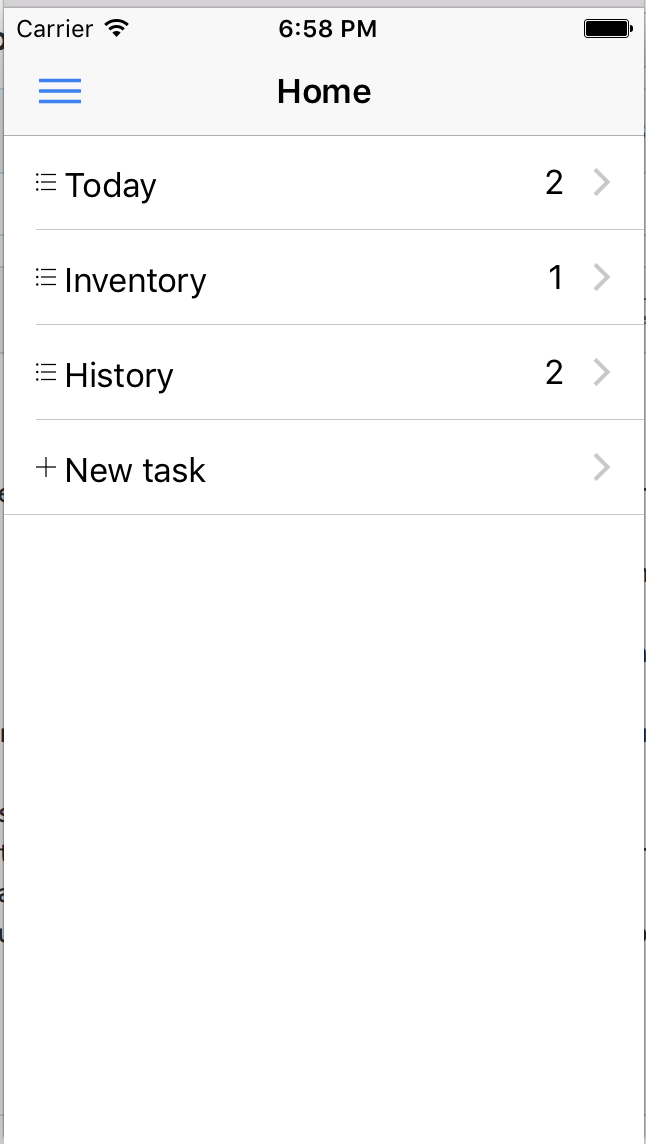
\includegraphics[width=10cm]{home}\\
		\caption{Home page}
		\label{jump}
	\end{figure}
	
	\begin{figure}[h]
		\centering
		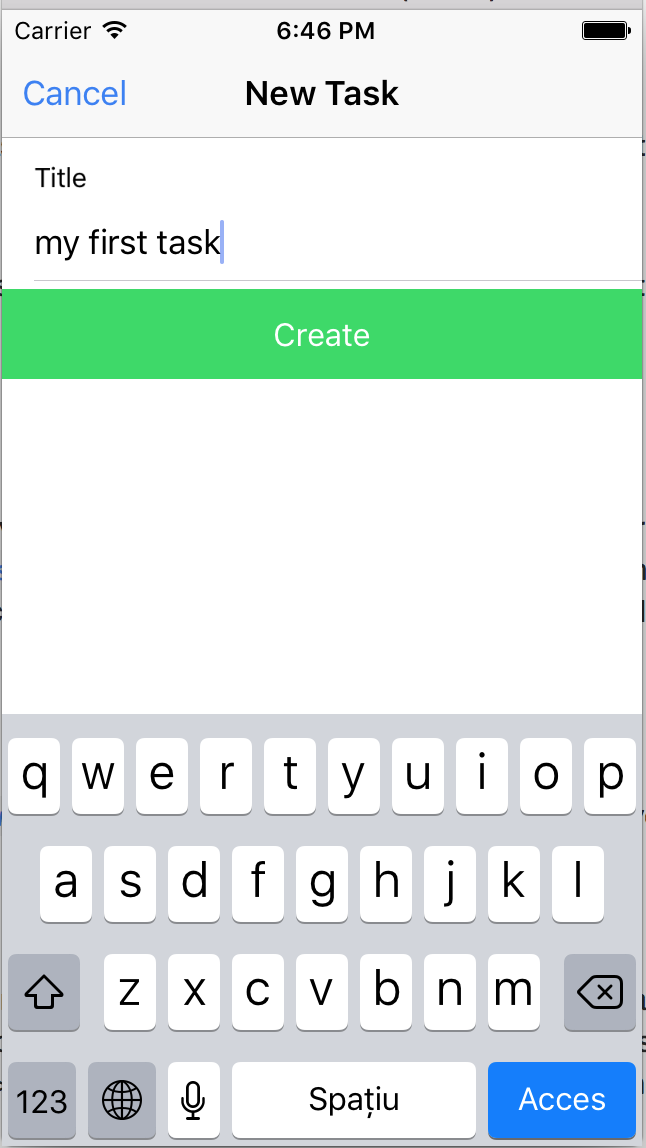
\includegraphics[width=10cm]{new-task}\\
		\caption{Create new task}
		\label{slide}
	\end{figure}
	
	\begin{figure}[h]
		\centering
		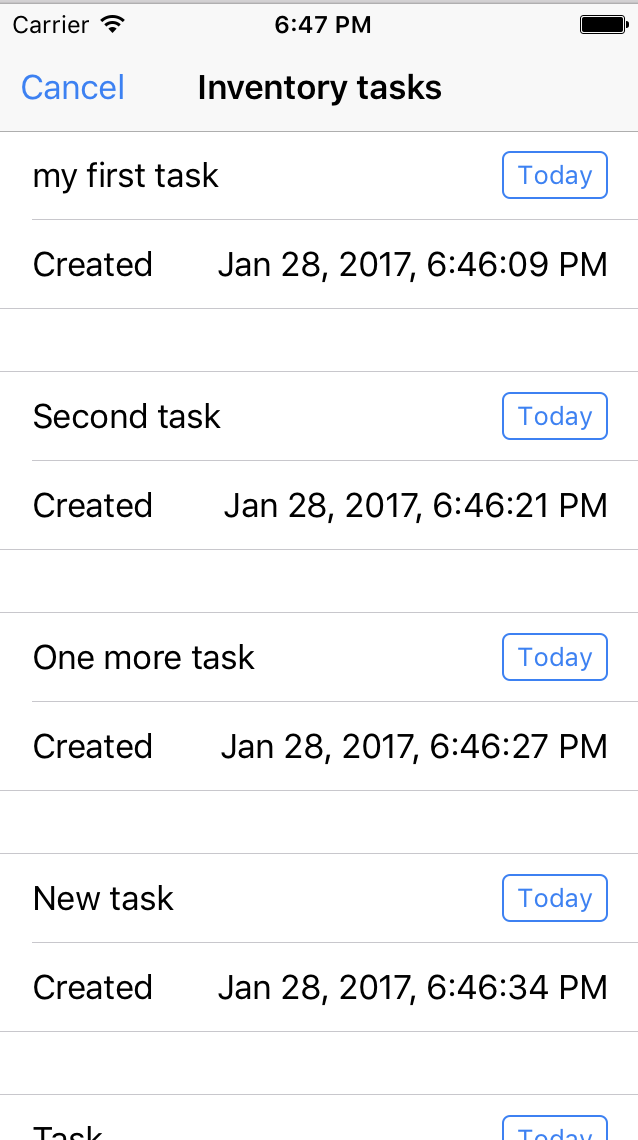
\includegraphics[width=10cm]{inventory}\\
		\caption{Inventory list}
		\label{lose}
	\end{figure}
	\begin{figure}[h]
		\centering
		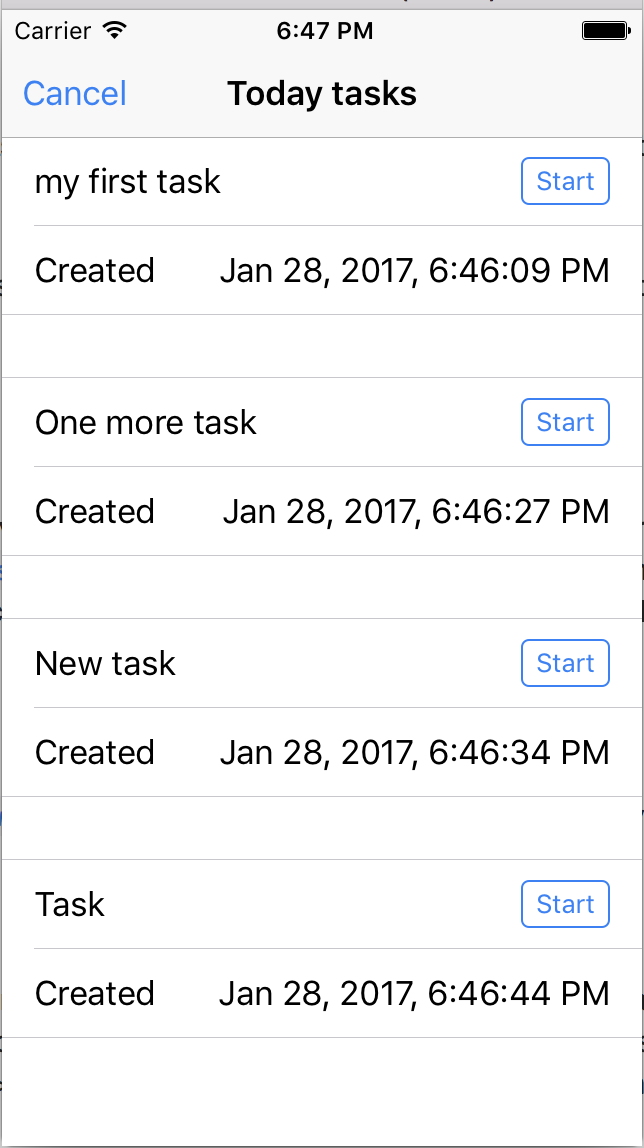
\includegraphics[width=10cm]{today}\\
		\caption{Today list}
		\label{jump}
	\end{figure}
	
	\begin{figure}[h]
		\centering
		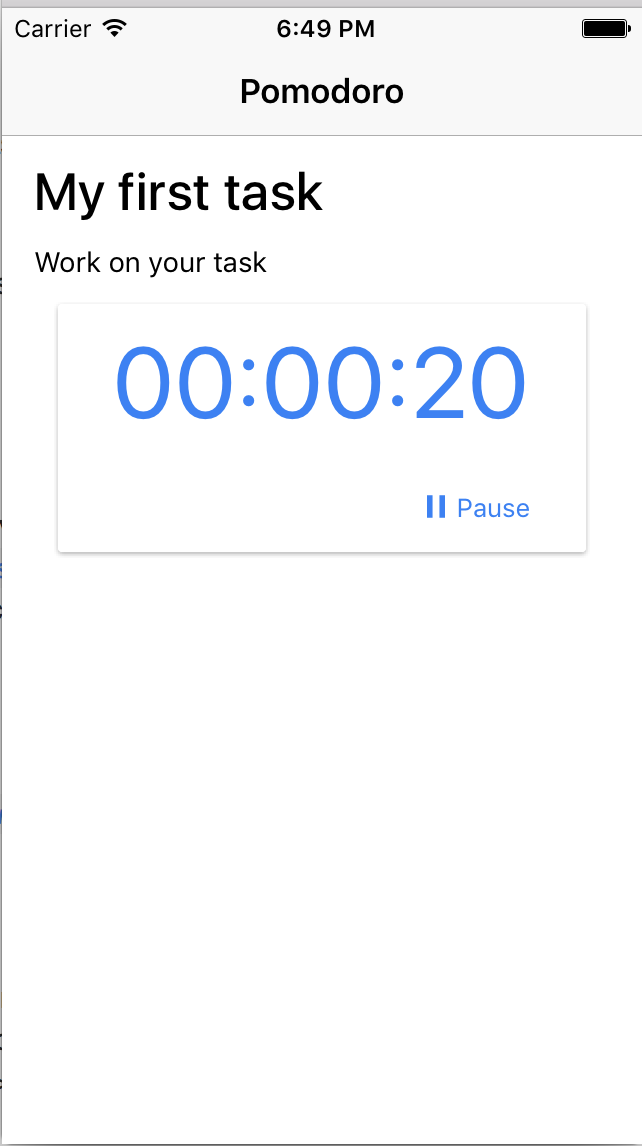
\includegraphics[width=10cm]{work-state}\\
		\caption{Promodoro}
		\label{slide}
	\end{figure}
	
	\begin{figure}[h]
		\centering
		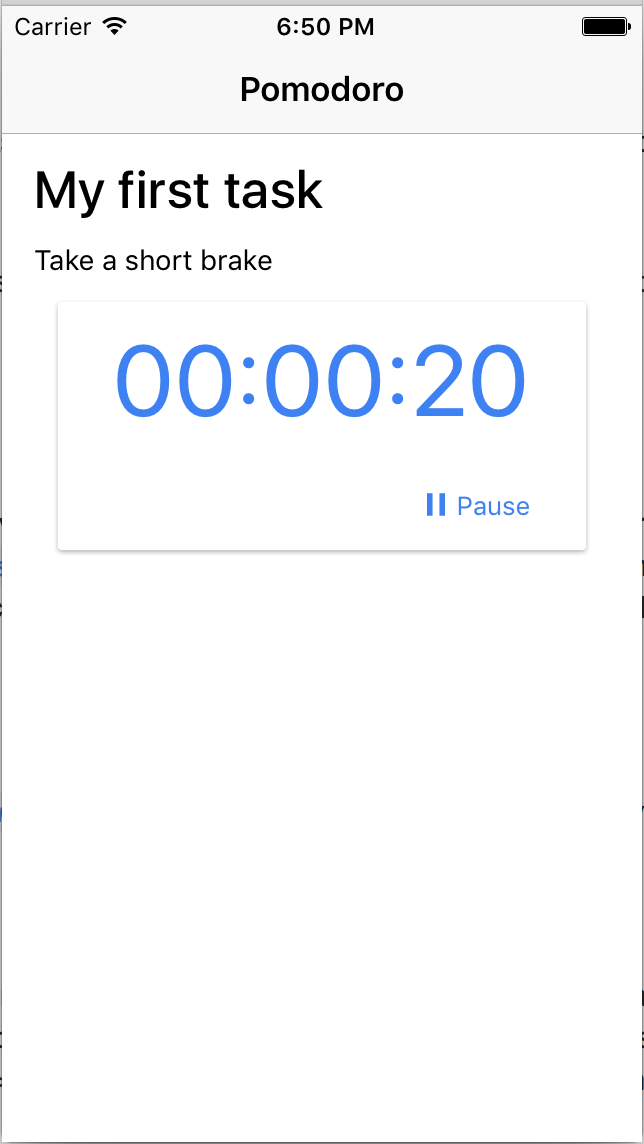
\includegraphics[width=10cm]{break-state}\\
		\caption{Break state}
		\label{lose}
	\end{figure}
	
	\begin{figure}[h]
		\centering
		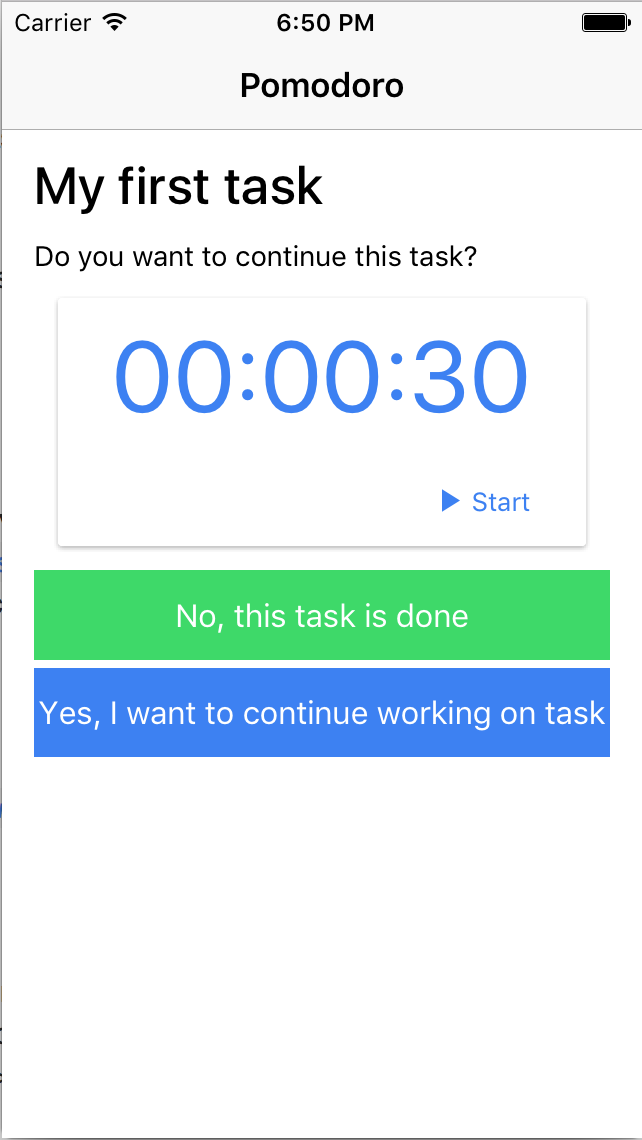
\includegraphics[width=10cm]{choose-state}\\
		\caption{Choose state}
		\label{jump}
	\end{figure}
	
	\begin{figure}[h]
		\centering
		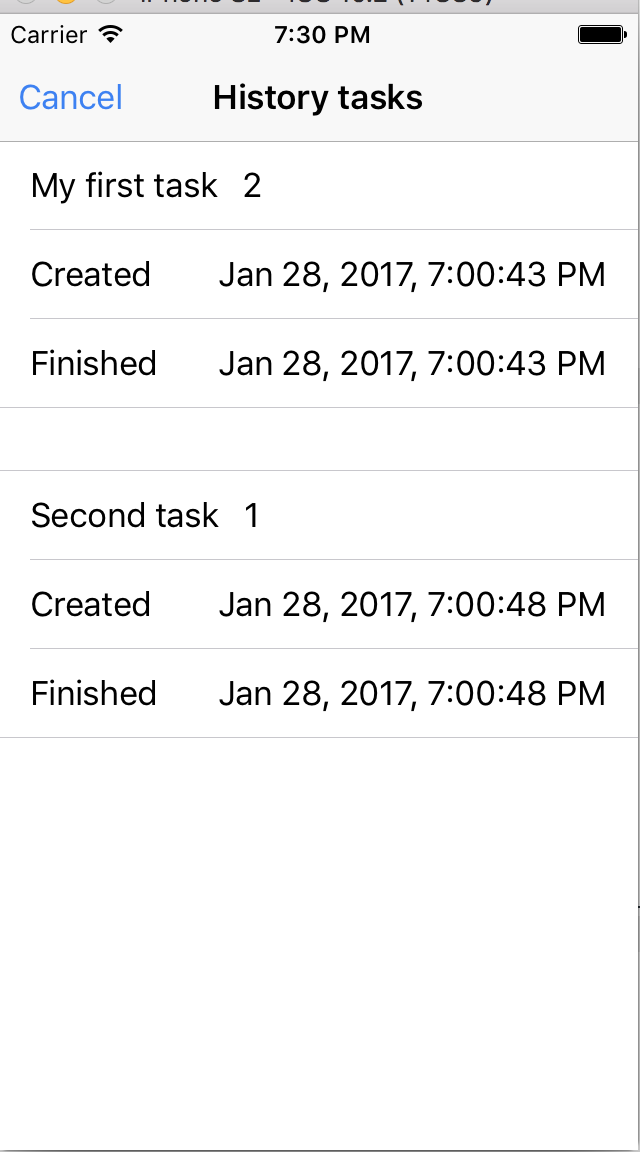
\includegraphics[width=10cm]{history}\\
		\caption{History List}
		\label{slide}
	\end{figure}
	
	\begin{figure}[h]
		\centering
		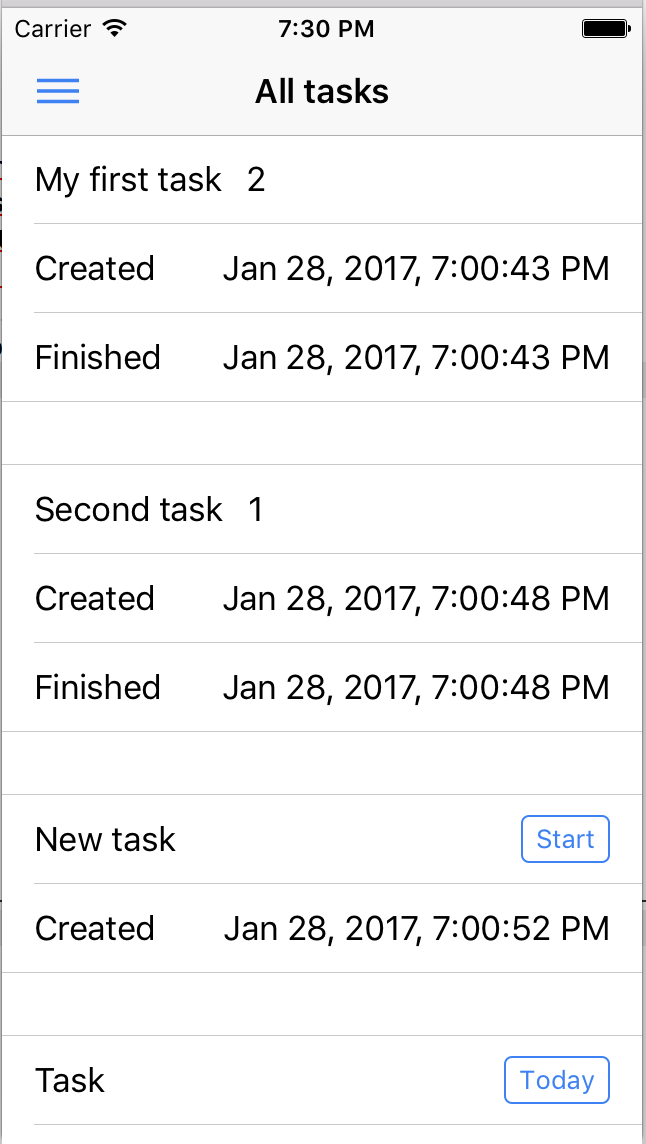
\includegraphics[width=10cm]{all}\\
		\caption{All List}
		\label{slide}
	\end{figure}
\end{center}

\clearpage